\section{Interaktive Benutzung von Vistra}
\label{benutzung}

Mit Vistra k"onnen Trainings- und Testdaten f"ur neuronale Netze
visualisiert, editiert und transformiert werden.
Bevor die Bedienung von Vistra beschrieben wird, soll zun"achst
einmal exakt definiert werden, was unter Trainings- bzw.~Testdaten
zu verstehen ist.
Trainings- oder Testdaten umfassen
\begin{itemize}
\item $n$ Eingabevektoren ($n \geq 1$) \\ 
Jedes Element eines Eingabevektors entspricht dem Aktivierungszustand einer
Eingabezelle eines neuronalen Netzes.
\item optional $n$ Ausgabevektoren \\
Jedes Element eines Ausgabevektors entspricht dem Ausgabewert einer
Ausgabezelle eines neuronalen Netzes.
\item optional $n$ Klassen \\
Eine Klasse wird entweder durch eine Nummer repr"asentiert oder
durch einen String, der den Namen einer bestimmten Ausgabeklasse darstellt.
\end{itemize}

Um mit Vistra bearbeitet werden zu k"onnen, m"ussen diese Daten den 
folgenden Bedingungen gen"ugen:

\begin{sloppypar}
\begin{itemize}
\item Alle Eingabevektoren besitzen die gleiche Dimensionalit"at $i$ 
($i \geq 1$).
\item Falls Ausgabevektoren existieren, ist jedem Eingabevektor genau
ein Ausgabevektor zugeordnet.
\item Alle Ausgabevektoren besitzen die gleiche Dimensionalit"at $o$
($o \geq 1$).
\item Falls Klassensymbole oder -nummern existieren, ist jedem 
Eingabevektor genau eine Klasse zugeordnet.
\item Es m"ussen Ausgabevektoren, Klassensymbole oder Klassennummern
vorhanden sein. 
\end{itemize}
\end{sloppypar}

Diese Bedingungen werden immer dann "uberpr"uft, wenn Trainingsvektoren 
aus einer Datei eingelesen werden.

\subsubsection*{Klassen-Nummern}

Vistra weist jedem Trainingsvektor intern eine bestimmte Klassennummer zu.
Die Klassennummern werden nach dem Laden der Trainingsvektoren aus
den Klassensymbolen oder den Ausgabevektoren errechnet.
Sie werden aufsteigend, beginnend bei 1, vergeben. 

Existieren Klassensymbole, so erh"alt jedes unterschiedliche Symbol
eine eigene Nummer.
Die gr"o"ste Klassennummer entspricht in diesem Fall der Anzahl der
verschiedenen Klassen.
Existieren keine Klassensymbole, so berechnet Vistra die Klassennummern
aus den Ausgabevektoren, indem gleiche Ausgabevektoren gleiche
Klassennummern erhalten.
Die Klassennummern werden in der Reihenfolge vergeben, in der die Klassensymbole
bzw. die Ausgabevektoren in der Trainingsvektor-Datei erscheinen.
  
{\bf Beispiel:} Das xor-Problem kennt die zwei Klassen NULL und EINS.
Die Klasse NULL erh"alt die Klassennummer~1 und die Klasse EINS die Nummer~2.
Die Trainingsvektoren haben hier also folgende Nummern:

\begin{tabular}{ccc}
{\it Eingabevektor} & {\it Klassensymbol} & {\it Klassennummer} \\[1ex]
{\tt 0.0 0.0} & {\tt NULL} & {\tt 1} \\
{\tt 0.0 1.0} & {\tt EINS} & {\tt 2} \\
{\tt 1.0 0.0} & {\tt EINS} & {\tt 2} \\
{\tt 1.0 1.0} & {\tt NULL} & {\tt 1}  
\end{tabular}

Klassennummern k"onnen "uber Symboltabellen in Klassensymbole "ubersetzt
werden.
Symboltabellen stellen also Abbildungen von Klassennummern nach
Klassensymbolen dar und sind in Symboltabellen-Dateien gespeichert. 
Die $i$-te Zeile dieser Dateien enth"alt das Symbol der Klasse 
mit der Nummer $i$ (siehe auch Abschnitt~\ref{symtab}).

Da Vistra Symboltabellen-Dateien sowohl lesen als auch schreiben kann,
ist es m"oglich, die Klassensymbole durch einen 
anderen Satz von Symbolen zu ersetzen bzw.~Symbole erst zu einem 
sp"ateren Zeitpunkt als die Trainingsvektoren zu laden.
Letzteres ist beispielsweise n"otig, wenn Trainingsvektoren im 
N01-Format gelesen wurden, da das N01-Format anstelle von Klassensymbolen
nur Klassennummern verwendet.
Die zugeh"origen Symbole m"ussen "uber eine Symboltabelle nachtr"aglich
geladen werden.
Die Klassennummer verr"at dabei, welches Symbol f"ur welchen Trainingsvektor
zu verwenden ist.

\subsection{Das Hauptfenster}

Abbildung~\ref{hauptfenster} zeigt das Hauptfenster von Vistra.
Es erscheint, wenn Vistra im interaktiven Modus aufgerufen wird.

\begin{figure}[ht]
\centerline{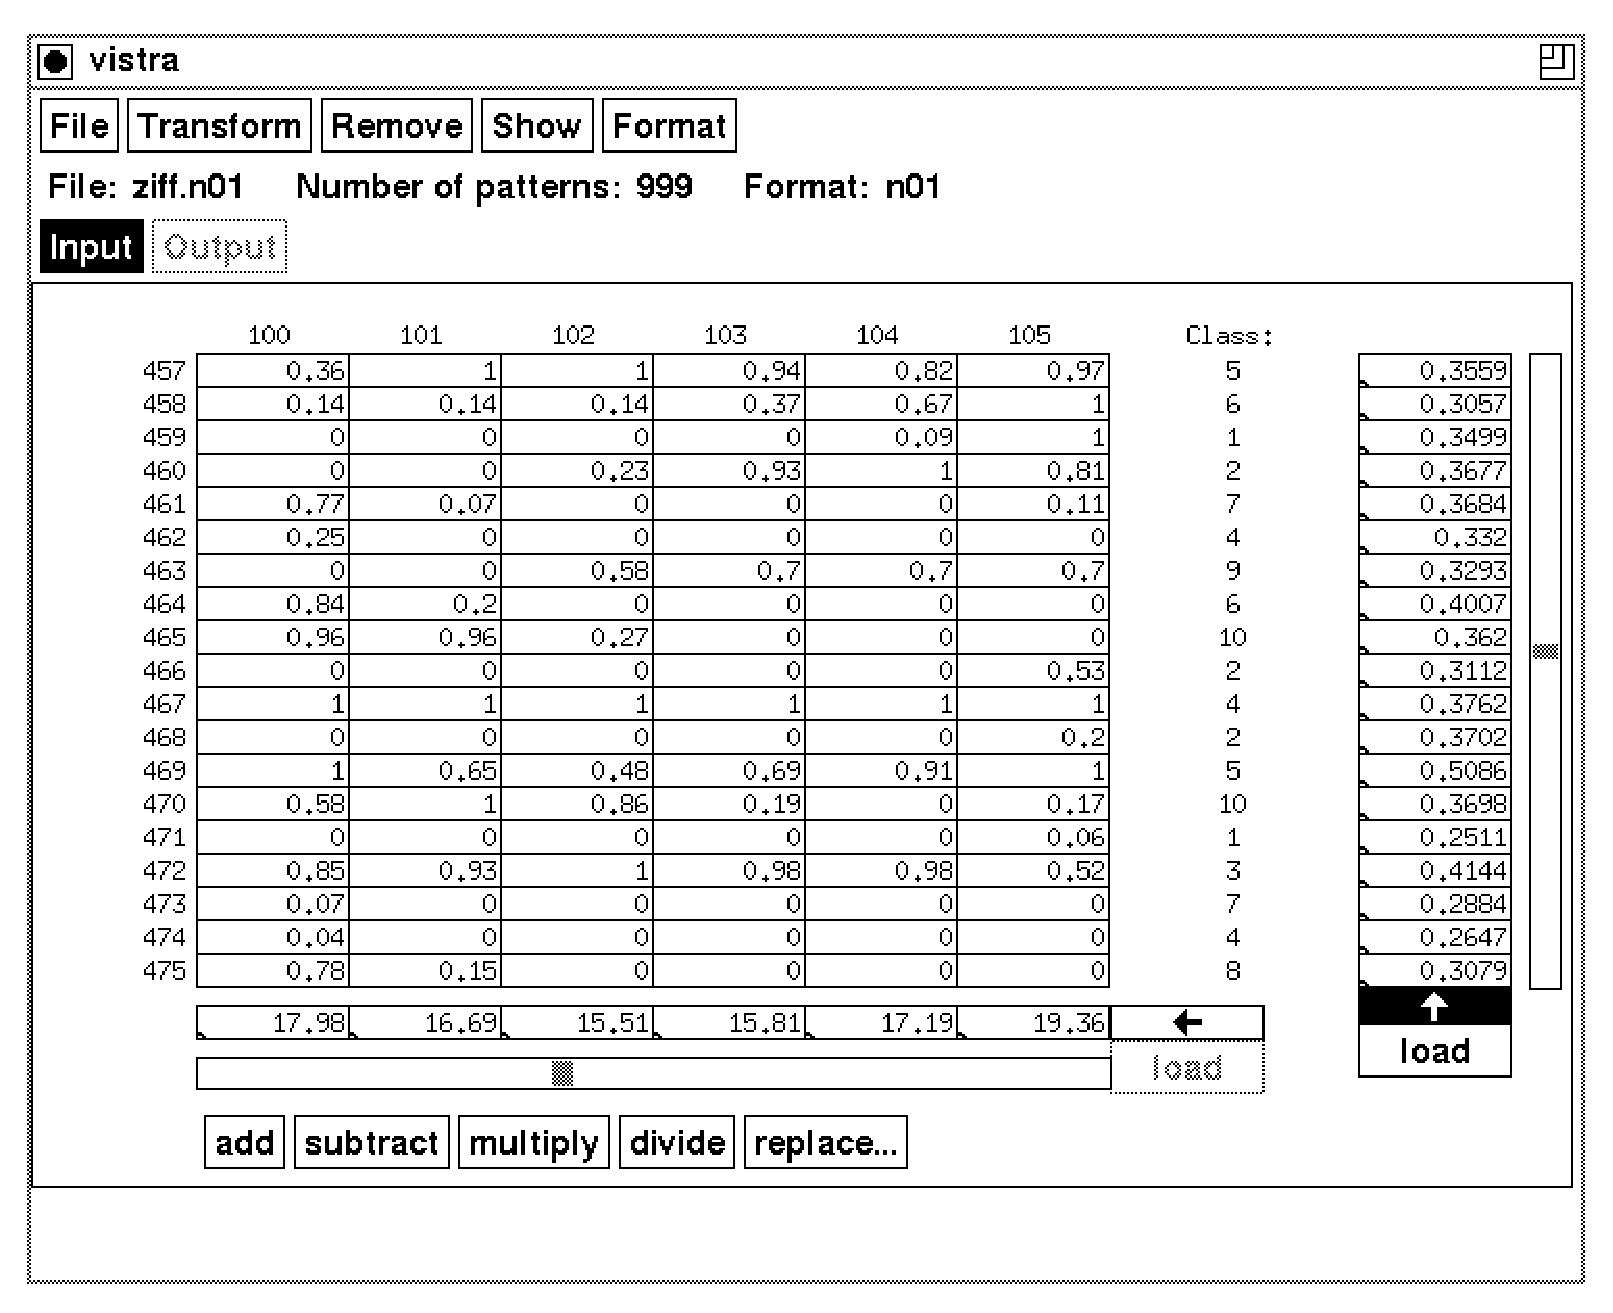
\psfig{file=main.ps,width=\textwidth,height=14cm}}
\caption{\label{hauptfenster} Das Hauptfenster von Vistra}
\end{figure}  

Das Hauptfenster ist in folgende Zonen eingeteilt:
\begin{itemize}
\item Direkt unter der Titelleiste befindet sich die {\bf Men"uleiste}, die
Men"u-Buttons f"ur das "`File"'-, "`Transform"'-, "`Remove"'-, "`Show"'- und 
"`Format"'-Men"u enth"alt.

\item Unterhalb der Men"uleiste folgt eine {\bf Info-Zeile}, die den Namen der
momentan geladenen Trainingsvektor-Datei, die Anzahl der Trainingsvektoren
sowie das momentan ausgew"ahlte Dateiformat anzeigt.

\item Es folgen {\bf zwei Buttons}, die mit "`Input"' bzw.~"`Output"' 
bezeichnet sind. 
Da im Hauptfenster immer nur ein Satz von Vektoren bearbeitet werden kann,
dienen diese Buttons zum Umschalten zwischen Eingabe- und Ausgabevektoren.
"Uber den Men"upunkt "`Input/output vectors"' des "`Show"'-Men"us
kann jedoch ein zweites Fenster ge"offnet werden, in dem immer diejenigen
Vektoren angezeigt werden, die momentan nicht im Hauptfenster bearbeitet 
werden (siehe auch Abschnitt~\ref{ssw}).
Ein Mausklick auf den "`Input"'- bzw. den "`Output"'-Button bewirkt 
ein Austauschen der beiden Fensterinhalte.

\item Ein {\bf Spreadsheet}, das entweder die Eingabe- oder die
Ausgabevektoren enth"alt.
Jede Zeile des Gitters entspricht einem Vektor.
Die Nummern der zum jeweiligen Zeitpunkt sichtbaren Vektoren sind
links neben dem Gitter angebracht.
Unmittelbar oberhalb des Gitters stehen die Nummern der sichtbaren
Dimensionen. \\
In Abbildung~\ref{hauptfenster} werden z.B. momentan die Dimensionen
100 bis 105 der Vektoren 457 bis 475 angezeigt.
Mithilfe der vertikalen bzw.~der horizontalen Scrollbars rechts 
bzw.~unterhalb des Gitters, k"onnen alle Vektorelemente bequem 
durchgebl"attert werden.

\begin{sloppypar}
Unmittelbar rechts neben dem Spreadsheet ist eine Spalte mit der
"Uberschrift "`class:"' zu sehen.
Sie enth"alt die Namen bzw.~Symbole der Klassen, denen die Vektoren
der entsprechenden Zeilen angeh"oren.
Sind keine Klassensymbole geladen, so sind an dieser Stelle die
zugeh"origen Klassennummern aufgef"uhrt. 
\end{sloppypar}

\item Direkt unterhalb bzw.~rechts neben dem Spreadsheet befinden sich 
{\bf horizontale bzw.~vertikale Skalarfelder}.
Sie dienen \ldots

\begin{enumerate}
\item zur Anzeige von Skalar-Werten, die aus den Zeilen-
bzw.~Spaltenvektoren des Spreadsheets abgeleitet werden.
Die vertikalen Felder werden dabei mit Skalaren gef"ullt, die
sich aus den Zeilenvektoren, also Eingabe- oder Ausgabevektoren,
ergeben.
Die horizontalen Felder beziehen sich hingegen auf die Spaltenvektoren
des Spreadsheets und enthalten daher Informationen "uber die einzelnen
Dimensionen der Vektoren.
\item als skalare Operanden zur Durchf"uhrung von Operationen
mit den Vektoren der Spreadsheet (Zeilen- oder Spaltenvektoren).
\end{enumerate}

Immer wenn neue Trainingsvektoren geladen werden bzw. von Eingabe- auf
Ausgabevektoren umgeschaltet wird (oder umgekehrt), werden alle 
vertikalen und horizontalen Skalarfelder auf den Wert "`0"' gesetzt.
Sp"ater k"onnen diese Felder auf zwei Arten mit Werten gef"ullt werden:

\begin{itemize}
\item von Hand mithilfe der Tastatur (dazu mu"s der Maus-Zeiger "uber
dem Eingabefeld stehen).
\item "uber einen Men"upunkt des "`Load"'-Men"us.
\end{itemize}

"Uber das "`Load"'-Men"u k"onnen Mittelwerte, Minima, Standardabweichungen
etc. von Vektoren oder Dimensionen berechnet werden.
Eine vollst"andige Liste der angebotenen Funktionen ist im
Abschnitt~\ref{loadmenu} zu finden.
Die Pfeile, die in Richtung der Skalarfelder zeigen, fungieren als
Schalter, mit denen zwischen den vertikalen und horizontalen Feldern
mittels Mausklick umgeschaltet wird.

Sind beispielsweise die vertikalen Felder selektiert, so beziehen sich
die Funktionen des "`Load"'-Men"us auf die Zeilen der Spreadsheet.
Die Minimum-Funktion des "`Load"'-Men"us w"urde die vertikalen Skalarfelder
mit dem jeweiligen minimalen Element des zugeh"origen Eingabe- bzw.
Ausgabevektors laden. 
Sind hingegen die horizontalen Felder ausgew"ahlt, so w"urden sie 
nach Ausf"uhrung der Minimum-Funktion die minimalen Elemente der einzelnen 
Dimensionen enthalten.

\item Mithilfe der {\bf Skalaroperations-Buttons} direkt unterhalb der 
horizontalen Scrollbar
werden die Zeilen- bzw.~Spaltenvektoren mit den Inhalten der vertikalen
bzw.~horizontalen Skalarfelder kombiniert.
Auch hier mu"s die Richtung der Operation vorher durch die Pfeile
eingestellt werden.
Sind die vertikalen Skalarfelder selektiert, so wird der $i$-te 
Zeilenskalar f"ur die Operation mit dem $i$-ten Zeilenvektor 
verwendet.
Sind hingegen die horizontalen Skalarfelder selektiert, so werden die
Spaltenskalare mit den Spaltenvektoren der Spreadsheet kombiniert.  
Folgende Vektor--Skalar Operationen sind m"oglich: 

\begin{tabular}{ll}
{\bf "`add"'} & elementweise Addition des Skalars \\
{\bf "`subtract"'} & elementweise Subtraktion des Skalars \\
{\bf "`multiply"'} & elementweise Multiplikation des Skalars \\
{\bf "`divide"'} & elementweise Division durch den Skalar \\
{\bf "`replace\ldots"'} & Ersetzen eines bestimmten Elements durch den Skalar \\
\end{tabular}

Im Falle von "`replace\ldots"' "offnet sich eine Dialogbox, in der
die Nummer des zu ersetzenden Elements angegeben werden mu"s.
Die "`replace\ldots"'-Funktion entspricht praktisch dem Ersetzen
einer Zeile bzw.~Spalte des Spreadsheets durch die Inhalte der horizontalen
bzw.~vertikalen Skalarfelder.

\item Der Platz unterhalb der Skalaroperations-Buttons dient zur
Anzeige von Mitteilungen "uber Operationen, Berechnungen usw., die
Vistra momentan durchf"uhrt.

"`Loading patterns\ldots"' beispielsweise besagt,
da"s Vistra zur Zeit eine Trainingsvektor-Datei einliest und deshalb
mit weiteren Benutzereingaben gewartet werden sollte.
\end{itemize}

Au"ser den Vektor--Skalar Operationen werden alle Aktionen des Hauptfensters
"uber entsprechende Men"upunkte aufgerufen.
Die folgenden Abschnitte beschreiben alle Aktionen Men"u f"ur Men"u. 
Generell gilt, da"s Operationen, deren Bezeichnungen auf "`\ldots"' enden, 
nicht sofort ausgef"uhrt werden, sondern zun"achst Dialogboxen "offnen,
in denen der Benutzer zus"atzliche Angaben zur Operation machen mu"s.  

\subsection{Das "`Load"'-Men"u}
\label{loadmenu}

Wie bereits erw"ahnt, dient das "`Load"'-Men"u zum Laden der
vertikalen oder der horizontalen Skalarfelder.
Mithilfe der beiden Pfeile k"onnen die zu ladenden Felder
ausgew"ahlt werden.
Unter jedem Pfeil befindet sich ein mit "`load"' gekennzeichneter
Men"ubutton, "uber den das "`Load"'-Men"u aufgerufen werden kann.

"Uber das "`Load"'-Men"u k"onnen sowohl skalare Werte zu den einzelnen
Vektoren bzw. Dimensionen bestimmt werden als auch globale Werte,
die von {\sl allen} Vektoren abh"angen (wie z.B. das minimale Element aller
Vektoren). 

Die ersten sieben Men"upunkte berechnen die Skalare aus den zugeh"origen
Zeilenvektoren (falls die vertikalen Felder selektiert sind), oder
aus den Spaltenvektoren des Spreadsheets
(falls die horizontalen Felder selektiert sind).  

\begin{samepage}
Sie lauten: \\
\begin{tabular}{lp{10.5cm}}
{\bf Men"upunkt} & {\bf geladen wird\ldots} \\[1ex]
"`minimum"' & das kleinste Element des Vektors \\
"`maximum"' & das gr"o"ste Element des Vektors \\
"`average"' & der Mittelwert der Vektorelemente \\
"`length"' & die L"ange des Vektors \\
"`standard deviation"' & die Standardabweichung $\sigma$ des 
Vektors $v$: \newline
\vspace{1ex}
\[ \sigma(v) = \sqrt{\frac{1}{dims} \sum_{i=1}^{dims} 
(v_{i} - \overline{v})^{2}} \]
\vspace{1ex}
\begin{tabbing}
$dims$ \qquad \= Dimensionalit"at von $v$ \\
$v_{i}$ \> $i$-tes Element von $v$ \\
$\overline{v}$ \> Mittelwert von $v$ 
\end{tabbing} \\
"`sum"' & die Summe aller Elemente des Vektors \\
"`pattern\ldots"' & das $i$-te Element des Vektors, wobei $i$ durch
den Benutzer in einer Dialogbox festgelegt wird 
\end{tabular}
\end{samepage}

Die n"achsten f"unf Men"upunkte f"ullen alle horizontalen bzw.~vertikalen
Skalarfelder mit einer Konstanten: \\

\nopagebreak
\begin{tabular}{lp{9.5cm}}
{\bf Men"upunkt} & {\bf geladen wird\ldots} \\[1ex]
"`overall minimum"' & das kleinste Element {\sl aller} Vektoren \\
"`overall maximum"' & das gr"o"ste Element {\sl aller} Vektoren \\
"`overall average"' & der Mittelwert der Elemente {\sl aller Vektoren} \\
"`overall std dev"' & die globale Standardabweichung $\sigma_{global}$
der Elemente {\sl aller} Vektoren $v_{i}$: \newline
\vspace{1ex}
\[ \sigma_{global} = \sqrt{\frac{1}{n\cdot dims} \sum_{i=1}^{n}
\sum_{j=1}^{dims} (v_{ij} - \overline{v})^{2}} \] 
\vspace{1ex}
\begin{tabbing}
$dims$ \qquad \= Dimensionalit"at der Vektoren $v_{i}$ \\
$n$ \> Anzahl der Vektoren in dem Spreadsheet \\
$v_{ij}$ \> $j$-tes Element des Vektors $v_{i}$ \\
$\overline{v}$ \> globaler Mittelwert ("`overall average"')      
\end{tabbing} \\
"`constant\ldots"' & eine beliebige Konstante, die vom Benutzer in einer 
Dialogbox eingegeben wird 
\end{tabular}

\subsection{Das "`Format"'-Men"u}

Vistra kann eine Vielzahl von Dateiformaten f"ur Trainingsvektoren lesen
und schreiben.
Neben dem LVQ- und dem N01-Format, die standardm"a"sig vorhanden sind,
handelt es sich um benutzerdefinierte ASCII-Formate, 
um die Vistra erweitert werden kann (wie in Kapitel~\ref{fdl} beschrieben).
Beim Lesen bzw.~Schreiben von Trainingsvektoren mu"s der Benutzer daher
das zu verwendende Format festlegen.
Dies geschieht "uber das "`Format"'-Men"u, in dem die Namen aller
dem Programm bekannten Formate aufgelistet sind.
 
Zu jedem Zeitpunkt ist ein Format selektiert und durch einen Haken links
vom Namen gekennzeichnet.
Zus"atzlich wird das ausgew"ahlte Format auch in der Info-Zeile angezeigt.
Die ersten drei Men"upunkte lauten "`see suffix"', "`lvq"' und "`n01"'.
"`see suffix"' bezeichnet hierbei kein bestimmtes Format, sondern legt fest, 
da"s das zu verwendende Format jeweils durch
die Endung des Dateinamens bestimmt ist.
Ist "`see suffix"' selektiert und soll z.B.~die Vektordatei "`ziffern.n01"'
geladen werden, so geht Vistra davon aus, da"s diese Datei im N01-Format
vorliegt.

Ab dem vierten Men"upunkt erscheinen die Namen der benutzerdefinierten
Formate.
Als Namen dienen hierbei die Dateinamen der FDL-Beschreibungen ohne
die Endung "`.fmt"'.  
 
\subsection{Das "`File"'-Men"u}

"Uber das "`File"'-Men"u k"onnen alle Vistra-Funktionen aufgerufen werden,
die mit dem Lesen oder dem Schreiben von Dateien zutun haben. 

\begin{description}
\item["`Load patterns\ldots"':] \mbox{} \\  
Lade neue Trainingsvektoren. \\
Es "offnet sich eine Dialogbox, in der der Name der Vektor-Datei
anzugeben ist.
Ist im "`Format"'-Men"u "`see suffix"' eingestellt, so gibt die Endung
des Dateinamens an, welches Format die Datei besitzt.

\item["`Write patterns\ldots"':] \mbox{} \\
Schreibe die bearbeiteten Trainingsvektoren in eine 
Trai\-nings\-vek\-tor-Datei. \\
Es "offnet sich eine Dialogbox, in der der Name der zu schreibenden Datei
anzugeben ist.
Ist im "`Format"'-Men"u "`see suffix"' eingestellt, so gibt die Endung
des Dateinamens an, in welchem Format die Trainingsvektoren geschrieben 
werden.

\item["`Load symbols\ldots"':] \mbox{} \\
Lade eine neue Symboltabelle. \\
Die Funktion ordnet den Klassennummern neue Symbole zu.
Die Symbole m"ussen dazu in einer Symboltabellen-Datei untergebracht sein.
Eine solche Symboltabellen-Datei hat Zeilenstruktur, wobei
die erste Zeile das erste Symbol enth"alt, die zweite Zeile das
zweite Symbol etc. 
Eine genaue Beschreibung des Formats findet sich im Abschnitt~\ref{symtab}.
Der Namen der Symboltabellen-Datei wird "uber eine Dialogbox vom Benutzer
erfragt.

Am Beispiel des xor-Problems soll dieser Proze"s veranschaulicht
werden. \\
Folgende Daten seien vor dem Laden im Speicher: 

\begin{tabular}{ccc}
{\sl Trainingsvektor} & {\sl Klassennummer} & {\sl Klassensymbol} \\[1ex]
{\tt 0 0} & {\tt 1} & {\tt NULL} \\
{\tt 0 1} & {\tt 2} & {\tt EINS} \\
{\tt 1 0} & {\tt 2} & {\tt EINS} \\
{\tt 1 1} & {\tt 1} & {\tt NULL} \\
\end{tabular}  

Die Symbole {\tt NULL} und {\tt EINS} sollen nun durch die Symbole
{\tt FALSE} und {\tt TRUE} ersetzt werden.
Dazu wird eine Symboltabellen-Datei mit folgendem Inhalt geladen: 
\begin{verbatim}
FALSE
TRUE
\end{verbatim}
Nach dem Laden liegen folgende Daten vor: 

\begin{tabular}{ccc}
{\sl Trainingsvektor} & {\sl Klassennummer} & {\sl Klassensymbol} \\[1ex]
{\tt 0 0} & {\tt 1} & {\tt FALSE} \\
{\tt 0 1} & {\tt 2} & {\tt TRUE} \\
{\tt 1 0} & {\tt 2} & {\tt TRUE} \\
{\tt 1 1} & {\tt 1} & {\tt FALSE} \\
\end{tabular}  

Mit der "`Load symbols\ldots"'-Funktion k"onnen Symbole nicht nur
ersetzt werden, sondern "uberhaupt erst einmal geladen werden.
Dies ist, wie bereits erw"ahnt, f"ur Trainingsvektoren sinnvoll, die 
im N01-Format geladen wurden, da das Format nur Klassennummern enth"alt.

Enth"alt eine Symboltabellen-Datei weniger Symbole als unterschiedliche
Klassen existieren, so erscheint eine Fehlermeldung.

\item["`Write symbols\ldots"':] \mbox{} \\
Schreibe die Symboltabelle in eine Symboltabellen-Datei. \\
Der Namen dieser Datei wird vom Benutzer "uber eine Dialogbox erfragt.
Ausgegeben werden die Klassensymbole oder, falls keine geladen sind,
die Ausgabevektoren (siehe Abschnitt~\ref{symtab}).
Existieren weder Symbole noch Ausgabevektoren, so werden einfach die
Klassennummern geschrieben.
  
\item["`Write to log file"':] \mbox{} \\ 
Dieser Men"upunkt stellt einen Schalter 
dar, wobei ein Haken anzeigt, ob die Funktion ein- oder abgeschaltet ist.
Solange sie eingeschaltet ist, werden alle Transformationen, die
auf den Eingabe- oder Ausgabevektoren durchgef"uhrt werden, in einer
LOG-Datei festgehalten.
Zu einem sp"ateren Zeitpunkt k"onnen die durchgef"uhrten Transformationen
dann mit denselben oder anderen Trainingsvektoren wiederholt werden.
Die Funktion kann w"ahrend einer Sitzung beliebig ein- oder ausgeschaltet
werden, wobei immer nur ans Ende der LOG-Datei angeh"angt wird.

Der Namen der LOG-Datei ist {\it pattern\_file\_name}{\tt\/.log},
wobei {\it pattern\_file\_name} den Namen der momentan  
geladenen Trainingsvektor-Datei repr"asentiert.
Sie wird daher in das Verzeichnis der Vektordatei gestellt.  
Das Format der LOG-Dateien wird ausf"uhrlich 
im Kapitel~\ref{log} behandelt.

\item["`Quit"':] \mbox{} \\
Beende Vistra.  
\end{description}

\subsection{Das "`Transform"'-Men"u}

Das "`Transform"'-Men"u enth"alt Funktionen zur Transformation der
Eingabevektoren oder der Ausgabevektoren, je nachdem, welche gerade
im Hauptfenster bearbeitet werden.
Es werden immer {\sl alle} Vektoren transformiert, das gezielte
Transformieren eines einzelnen Vektors ist weder zweckm"a"sig noch erlaubt. \\ 
Folgende Transformationen sind m"oglich:

\begin{description}
\item["`HLOG"':] \mbox{} \\
Es wird eine halblogarithmische 
Transformation mit den Vektoren durchgef"uhrt. \\
Sie kann nur auf Vektoren ausgef"uhrt werden, die eine quadratische
Anzahl von Dimensionen besitzen. 

Bei der Bilderkennung mit Hilfe neuronaler Netze bereiten gedrehte Objekte
besonders gro"se Probleme.
Eine Abhilfe kann die sogenannte halblogarithmische Transformation 
schaffen.
Die Vektorelemente (Bildpunkte) werden durch diese Transformation nicht
ver"andert, sondern lediglich anders angeordnet.

Man kann sich die Transformation folgenderma"sen vorstellen: \\
Man legt $b$ konzentrische Kreise mit exponentiell wachsenden Radien um den
Mittelpunkt des Bildes, wobei $b$ die Seitenl"ange des quadratischen Bildes 
in Bildpunkten ist.
Der Radius $r_i$ des $i$-ten Kreises ($i=0,1,\ldots,b-1$) betr"agt:

\[ r_i = \left( \frac{b}{2}\right)^{\frac{i}{b-1}} \qquad \mbox{Bildpunkte} \] 

Legt man nun Geraden durch den Mittelpunkt, die jeweils einen Winkel
von $\frac{2\pi}{b}$ ein\-schlie"sen, so wird die erste Spalte des neuen
Bildes aus den Bildpunkten des Originals gebildet, die im 
Gegenuhrzeigersinn unter den Schnittpunkten dieser Geraden mit dem innersten
Kreis liegen.
Die zweite Spalte erh"alt man aus den Schnittpunkten mit dem zweitinnersten 
Kreis usw.
Die Schnittpunkte mit dem "au"sersten Kreis liefern schlie"slich die Elemente 
der letzten Spalte des transformierten Bildes. 

Durch die halblogarithmische Transformation wird erreicht, da"s
Drehungen von Objekten im Original   
zu Verschiebungen im transformierten Bild f"uhren.
Verschiebungen k"onnen von neuronalen Netzen jedoch wesentlich leichter
erkannt werden.

\item["`FFT"':] \mbox{} \\
Es wird eine diskrete eindimensionale 
Fourier Transformation (FFT) auf den Vektoren durchgef"uhrt.
Diese Transformation ist nur f"ur Vektoren zul"assig, die $2^{n}$ 
($n \geq 1$) Dimensionen besitzen.

Bei der FFT handelt es sich um eine komplexwertige Vektorfunktion.
Bevor eine FFT auf einem Vektor $v$ durchgef"uhrt wird, m"ussen die
Vektorelemente $v_{i}$ deshalb zun"achst in komplexe Zahlen 
$(v_{i,real},v_{i,imag})$ "uberf"uhrt werden. \\
Dies geschieht in Vistra wie folgt:

\begin{tabular}{@{\hspace*{1cm}}lcl}
$v_{i,real}$ & := & $v_{i}$ \\
$v_{i,imag}$ & := & $0.0$ \\
\end{tabular}

Nach Durchf"uhrung der Fourier Transformation auf dem Vektor $v$
werden die komplexen Vektorelemente wieder in reelle Zahlen umgewandelt:

\hspace*{1cm} $v_{i} := \sqrt{v_{i,real}^{2} + v_{i,imag}^{2}}$

Die diskrete eindimensionale Fourier Transformation ist ausf"uhrlich
in \cite{jaehne} beschrieben. 

\item["`PCA"':] \mbox{} \\ 
Auf den Vektoren wird eine 
Haupt\-achsen-Trans\-form\-ation 
({\bf P}rinciple {\bf C}om\-po\-nent {\bf A}na\-ly\-sis) 
durchgef"uhrt. \\
F"ur eine Beschreibung sei auf \cite{hertz} oder \cite{bronstein} verwiesen. 

Vistra verwendet zur Durchf"uhrung der PCA-Transformation das 
Programm "`pca"', das Trainingsvektoren im LVQ-Format liest, die PCA
durchf"uhrt und die transformierten Vektoren anschlie"send im LVQ-Format 
nach stdout schreibt. 

Vistra schreibt daher in einem ersten Schritt die Trainingsvektoren 
im LVQ-Format in eine tempor"are Datei, ruft anschlie"send das Programm 
"`pca"' mit dieser Datei als Parameter auf, lenkt die Ausgabe auf 
eine weitere tempor"are Datei um und liest diese 
schlie"slich wieder im LVQ-Format ein.

\item["`Normalize"':] \mbox{} \\
Alle Vektoren des Spreadsheets werden 
normalisiert, d.h.~jeder Vektor $v$ 
wird elementweise durch seine L"ange $|v|$ dividiert, so da"s jeder Vektor
anschlie"send die L"ange $|v|=1$ besitzt:
 
\[ v := \frac{v}{|v|} \]

Diese Transformation kann auch leicht mithilfe der Skalarfelder 
durchgef"uhrt werden.
Zuerst l"adt man die vertikalen Skalarfelder mit den L"angen der Vektoren
(Men"upunkt "`length"' des "`Load"'-Men"us).
Anschlie"send wird der "`divide"'-Button gedr"uckt.

\item["`Scale\ldots"':] \mbox{} \\
Die Elemente aller Vektoren werden 
auf einen neuen Wertebereich skaliert, der in einer Dialogbox anzugeben ist. 

Die Skalierung erfolgt derart, da"s das kleinste Element des Spreadsheets
("`overall minimum"') auf die untere Intervallgrenze und das gr"o"ste
("`overall maximum"') auf die obere Intervallgrenze abgebildet wird.

\item["`Randomize"':] \mbox{} \\
Die Reihenfolge der Trainingsvektoren wird willk"urlich ver"andert.

\item["`Expand with class vector"':] \mbox{} \\
Jeder Vektor des Spreadsheets wird mit seinem Klassenvektor erweitert. 

Unter Klassenvektor versteht man dabei einen Vektor bestehend aus Nullen
und Einsen, wobei die Anzahl der Dimensionen der Anzahl unterschiedlicher
Klassen entspricht. 
Das $i$-te Element des Klassenvektors ist genau dann 1, wenn der
Trainingsvektor die Klassennummer $i$ besitzt, sonst 0. 

Das Erweitern durch die Klassenvektoren soll am xor-Beispiel veranschaulicht
werden. \\
Links sind die Vektoren vor und rechts nach der Transformation zu
sehen: 

\nopagebreak
\begin{tabular}{ccc}
{\sl Eingabevektoren vorher} & {\sl Klassen-Nr.} & 
{\sl Eingabevektoren nachher} \\[1ex] 
{\tt 0 0} & {\tt 1} & {\tt 0 0 1 0} \\  
{\tt 0 1} & {\tt 2} & {\tt 0 1 0 1} \\  
{\tt 1 0} & {\tt 2} & {\tt 1 0 0 1} \\  
{\tt 1 1} & {\tt 1} & {\tt 1 1 1 0} \\  
\end{tabular}
 
\item["`Expand with output vector"':] \mbox{} \\
Diese Transformation kann nur durchgef"uhrt werden, wenn 
Ausgabevektoren existieren.
Die Vektoren des Spreadsheets werden mit den Elementen des 
zugeh"origen Ausgabevektors erweitert.

\item["`Refresh class numbers"':] \mbox{} \\
Es werden die Klassennummern anhand der Ausgabevektoren neu berechnet. \\ 
Diese Funktion kann nur aufgerufen werden, wenn keine Klassensymbole geladen
sind.

Trainingsvektoren mit gleichen Ausgabevektoren erhalten die gleichen
Klassennummern.
Die vergebenen Nummern sind 1, 2,\ldots, $n$ , wobei $n$ 
der Anzahl unterschiedlicher Ausgabevektoren entspricht.
\end{description}
 
\subsection{Das "`Remove"'-Men"u}

Das "`Remove"'-Men"u h"alt Funktionen bereit, mit denen Trainingsvektoren
oder bestimmte Dimensionen der Vektoren entfernt werden k"onnen:

\begin{description}
\item["`Dimensions\ldots"':] \mbox{} \\
Es wird ein Bereich von Dimensionen (also Spalten des Spreadsheets) entfernt. \\
Dazu "offnet sich eine Dialogbox, in der die erste und die letzte der
zu entfernenden Dimensionen anzugeben ist.
Es k"onnen nicht alle Dimensionen entfernt werden.

\item["`Constant dims"':] \mbox{} \\
Es werden alle konstanten Dimensionen, also alle Spalten des
Spread\-sheets, 
in denen alle Elemente die gleichen Werte besitzen, entfernt.
Sind alle Dimensionen konstant, so kann die Operation nicht
ausgef"uhrt werden.

\item["`Vectors\ldots"':] \mbox{} \\
Es wird eine Reihe von Trainingsvektoren entfernt. \\
In einer Dialogbox ist der Nummernbereich der zu entfernenden Vektoren
zu spezifizieren.
Es k"onnen jedoch nicht alle Trainingsvektoren gel"oscht werden.
\end{description}

\subsection{Das "`Show"'-Men"u} 

Neben dem Hauptfenster existieren weitere Fenster, die alle "uber
einen entsprechenden Men"upunkt des "`Show"'-Men"us ge"offnet werden. \\
Folgende Men"upunkte stehen zur Verf"ugung:

\nopagebreak
\begin{description}
\item["`Graphics"':] \mbox{} \\
Es wird ein Graphik-Fenster ge"offnet. 
Ein Graphik-Fenster kann wahlweise die Ein\-ga\-be- oder die Ausgabevektoren
in einer von f"unf verschiedenen Darstellungsarten graphisch darstellen.
Es k"onnen beliebig viele solcher Graphik-Fenster ge"offnet werden.
Dadurch ist es m"oglich, ein und denselben Vektor 
auf mehrere Arten gleichzeitig wiederzugeben.
   
\item["`Statistics"':] \mbox{} \\
Es wird ein Fenster ge"offnet, das statistische Informationen "uber die
geladenen Trai\-nings\-vek\-to\-ren anzeigt.

\item["`Covariance matrix"':] \mbox{} \\
Es wird ein Fenster ge"offnet, 
das die Kovarianzmatrix der im Hauptfenster befindlichen Vektoren
anzeigt.

\item["`Input/output vectors"':] \mbox{} \\
Es wird ein Fenster ge"offnet, in dem die Eingabevektoren oder die
Ausgabevektoren textuell dargestellt werden. 
Dieses Fenster enth"alt immer genau diejenigen Vektoren, die momentan
nicht im Hauptfenster bearbeitet werden.
Auf diese Weise k"onnen zugeh"orige Eingabe- und Ausgabevektoren
gleichzeitig betrachtet werden.
\end{description}

Die folgenden Abschnitte zeigen diese Fenster nun der Reihe nach und
geben Hinweise zu deren Benutzung.
  
\subsection{Die Graphik-Fenster}

Zu jedem Zeitpunkt k"onnen mehrere Graphik-Fenster ge"offnet sein.
Jedes dieser Fenster kann Vektoren in einer der folgenden f"unf
Darstellungsarten graphisch wiedergeben:

\begin{itemize}
\item als Histogramm
\item als Linienzug
\item als Grauwertbild
\item als Farbbild
\item als 2-dimensionale Projektion
\end{itemize} 

Zwischen diesen Darstellungsarten kann beliebig umgeschaltet werden.
Auch die Gr"o"se der Abbildungen kann man innerhalb gewisser Grenzen
ver"andern.
Abbildung~\ref{grayMat} zeigt ein Graphik-Fenster, das momentan 
auf "`gray matrix"' eingestellt ist und einen Vektor als Grauwertbild
darstellt.

\begin{figure}[ht]
\centerline{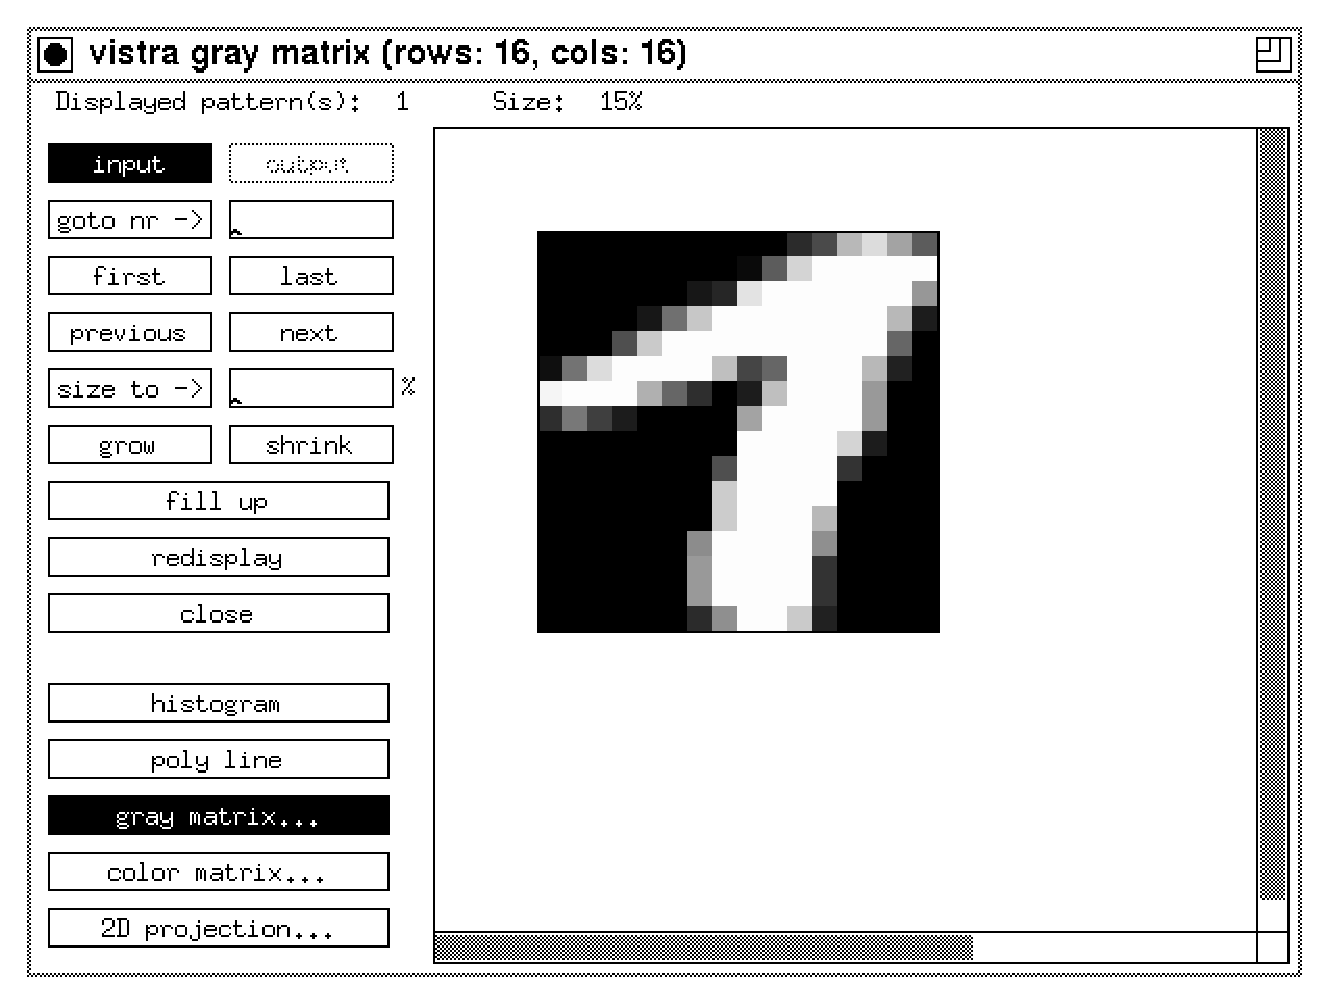
\psfig{file=gray.ps,width=\textwidth,height=10cm}}
\caption{\label{grayMat} Graphik-Fenster mit Grauwertbild}
\end{figure}

Der Titel des Fensters gibt an, welche Darstellungsart momentan gew"ahlt ist.
Unterhalb der Titelleiste erscheint eine Zeile, die Auskunft "uber die
Nummer des abgebildeten Vektors und die Gr"o"se der Abbildung (in \%
der Maximalgr"o"se) gibt.
F"ur die 2-dimensionale Projektion wird anstelle einer Vektor-Nummer
der String "`all"' angezeigt, da diese Darstellungsart alle Vektoren
gemeinsam in einer einzigen Graphik bzw.~Koordinatensystem wiedergibt. 

Am linken Rand des Graphik-Fensters befinden sich eine Reihe von 
Kommando-Buttons.
Durch sie werden Aktionen zum "`Durchbl"attern"' der Vektoren, zur
Ver\-gr"o"ser\-ung/Ver\-kleiner\-ung der Darstellungen oder zum Umschalten
zwischen Eingabe- und Ausgabevektoren bzw.~zum Umschalten zwischen den
verschiedenen Darstellungsarten, ausgef"uhrt. \\
Tabelle~\ref{gwcomms} beschreibt die Buttons des Graphik-Fensters.

\begin{table}[ht]
\begin{tabular}{lp{10.8cm}}
{\bf Button} & {\bf Aktion} \\ \hline
"`input"' & zeige einen Eingabevektor \\
"`output"' & zeige einen Ausgabevektor \\
"`goto nr --$>$"' & zeige den Vektor mit der Nummer, die das Eingabefeld rechts
daneben enth"alt \\
"`first"' & zeige den Vektor Nummer~1 \\
"`last"' & zeige den Vektor mit der h"ochsten Nummer \\
"`previous"' & zeige den vorhergehenden Vektor \\
"`next"' & zeige den n"achsten Vektor \\
"`size to --$>$"' & zeichne die Graphik in $i$ Prozent der Maximalgr"o"se, wobei
$i$ ins Eingabefeld rechts daneben einzutragen ist \\
"`grow"' & vergr"o"sere die Graphik \\
"`shrink"' & verkleinere die Graphik \\
"`fill up"' & nutze den Platz rechts und unterhalb des Diagramms zur 
gleichzeitigen Darstellung weiterer Vektoren.
"Uber jedem Diagramm befindet sich die Nummer des dargestellten Vektors.
Abbildung~\ref{fillup} zeigt ein Graphik-Fenster, das die Vektoren 1 bis 999
als Grauwertbilder minimaler Gr"o"se wiedergibt (1 Pixel pro Vektorelement).
  \\
"`redisplay"' & aktualisiere die Graphik (die dargestellten Vektoren
wurden im Hauptfenster seit dem letzten Zeichnen evtl.~modifiziert;
die graphische Darstellung w"are in diesem Fall veraltet) \\
"`close"' & schlie"se das Graphik-Fenster \\
"`histogram"' & zeige den Vektor als Histogramm \\
"`poly line"' & zeige den Vektor als Linienzug \\
"`gray matrix\ldots"' & zeige den Vektor als Grauwertbild. 
Die Anzahl der Zeilen und Spalten wird "uber eine Dialogbox durch den 
Benutzer festgelegt. \\
"`color matrix\ldots"' & zeige den Vektor als Farbbild.
Die Anzahl der Zeilen und Spalten wird "uber eine Dialogbox durch den
Benutzer festgelegt. \\
"`2D projection\ldots"' & stelle alle Vektoren in einem gemeinsamen
2-dimensionalen Koordinatensystem dar.
Der Benutzer legt in einer Dialogbox fest, welche Dimension die x-Werte
und welche Dimension die y-Werte liefern soll. 
\end{tabular}
\caption{\label{gwcomms} Die Buttons des Graphik-Fensters}
\end{table}

\begin{figure}[ht]
\centerline{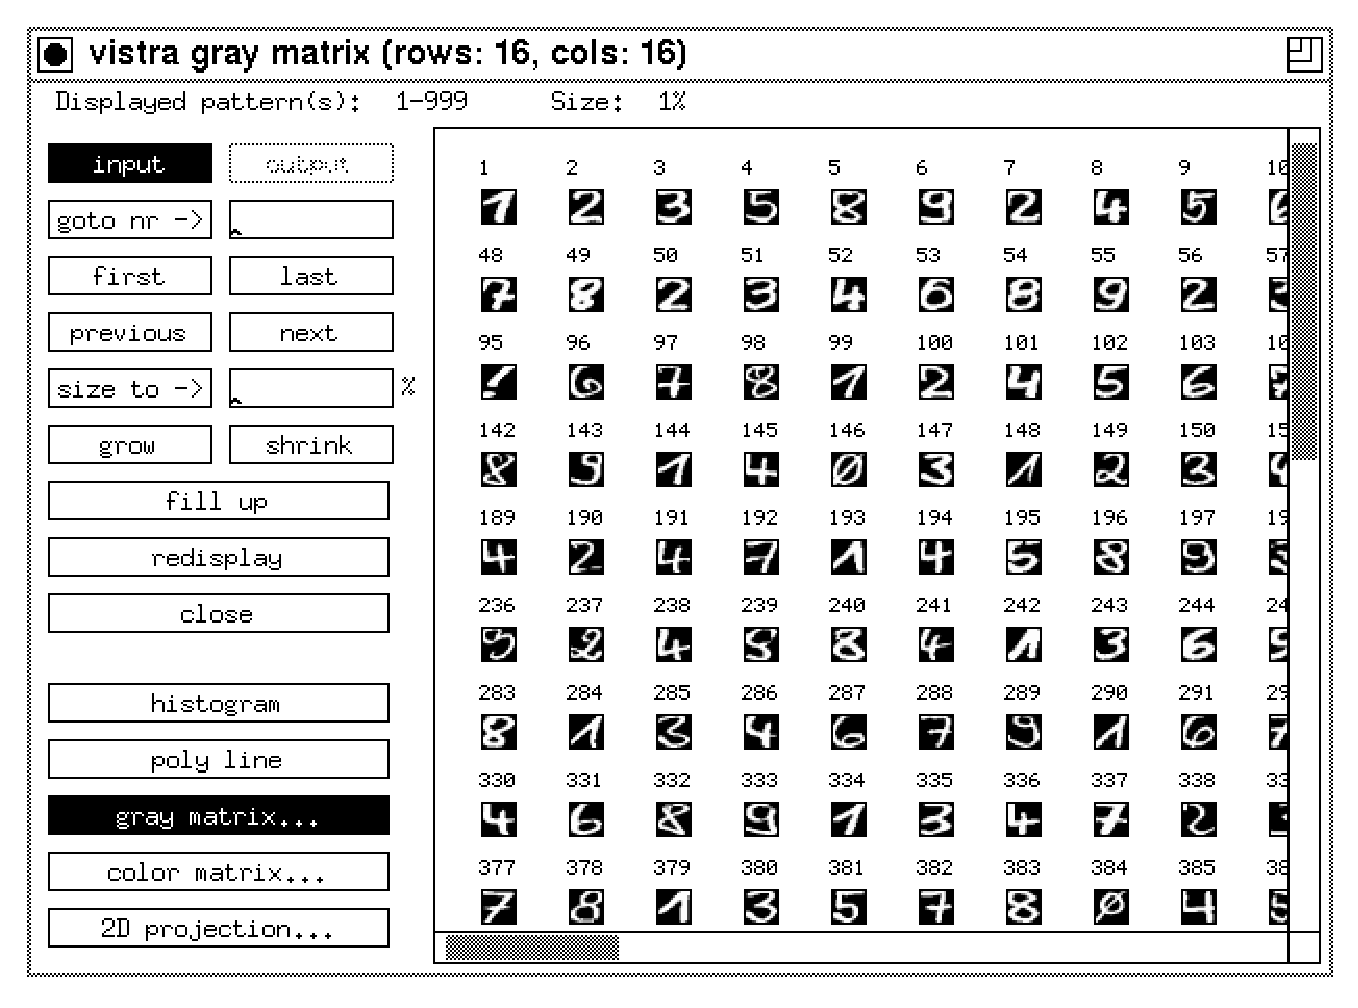
\psfig{file=fillup.ps,width=\textwidth,height=10cm}}
\caption{\label{fillup} Gleichzeitige Darstellung mehrerer Vektoren}
\end{figure}

{\bf WICHTIG:} Auch w"ahrend ein oder mehrere Graphik-Fenster ge"offnet 
sind, k"onnen die Vektoren im Hauptfenster weiterhin bearbeitet
bzw.~transformiert werden.
Aus diesem Grund ist es m"oglich, da"s ein Graphik-Fenster eine 
"`alte Version"' eines Vektors wiedergibt. 
Um sicherzustellen, da"s die Darstellung auf dem neuesten Stand ist,
sollte ein "`redisplay"' durchgef"uhrt werden oder irgendein anderer
Button gedr"uckt werden, der ein Neuzeichnen der Graphik bewirkt
(z.B.~"`next"', "`grow"' etc.). 

\subsection{Die Darstellungsarten}

\subsubsection*{Histogramm}

Ein Histogramm stellt eine Art "`Treppenfunktion"' in einem 
zweidimensionalen Koordinatensystem dar. 
Dabei liefert jedes Element $v_{i}$ des Vektors den Funktionswert 
f"ur den Bereich $[i\!-\!1,i]$ der x-Achse.
Abbildung~\ref{histo} zeigt ein Graphik-Fenster, das ein
Histogramm wiedergibt.
Der dargestellte Vektor besitzt 32 Dimensionen und ist das Ergebnis
einer vorausgegangen Fourier-Transformation.

\begin{figure}[ht]
\centerline{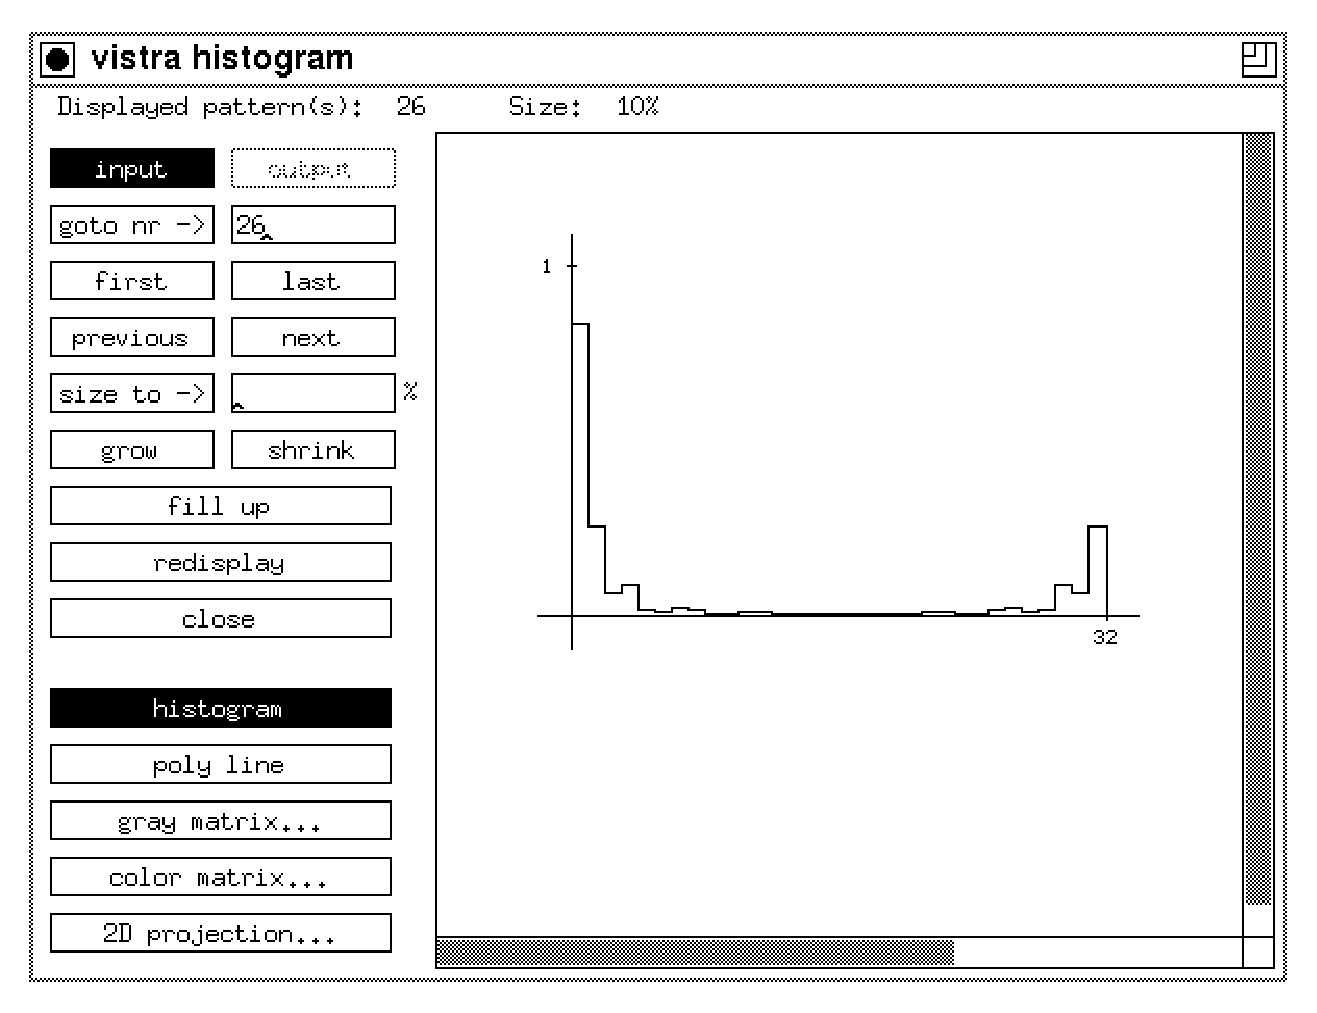
\psfig{file=histo.ps,width=\textwidth,height=10cm}}
\caption{\label{histo} Histogramm-Darstellung eines Vektors}
\end{figure} 

W"ahrend die H"ohe des Histogramms konstant bleibt, kann die Breite
"uber die entsprechenden Buttons des Graphik-Fensters ("`size to --$>$"',
"`grow"' oder "`shrink"') ver"andert werden.
Um die minimale Breite zu erhalten, gibt man als Gr"o"se "`0\%"' an.
Eine L"angeneinheit der x-Achse ist dann 1~Pixel breit.
 
\subsubsection*{Linienzug}

Ein Linienzug ist einem Histogramm sehr "ahnlich. 
Auch er wird in ein zweidimensionales Koordinatensystem gezeichnet.
Die Vektorelemente $v_{i}$ liefern dabei die Punkte $(i,v_{i})$, die
durch Linien verbunden werden.
Abbildung~\ref{poly} zeigt eine Linienzug-Darstellung des Vektors aus
Abbildung~\ref{histo}.

\begin{figure}[ht]
\centerline{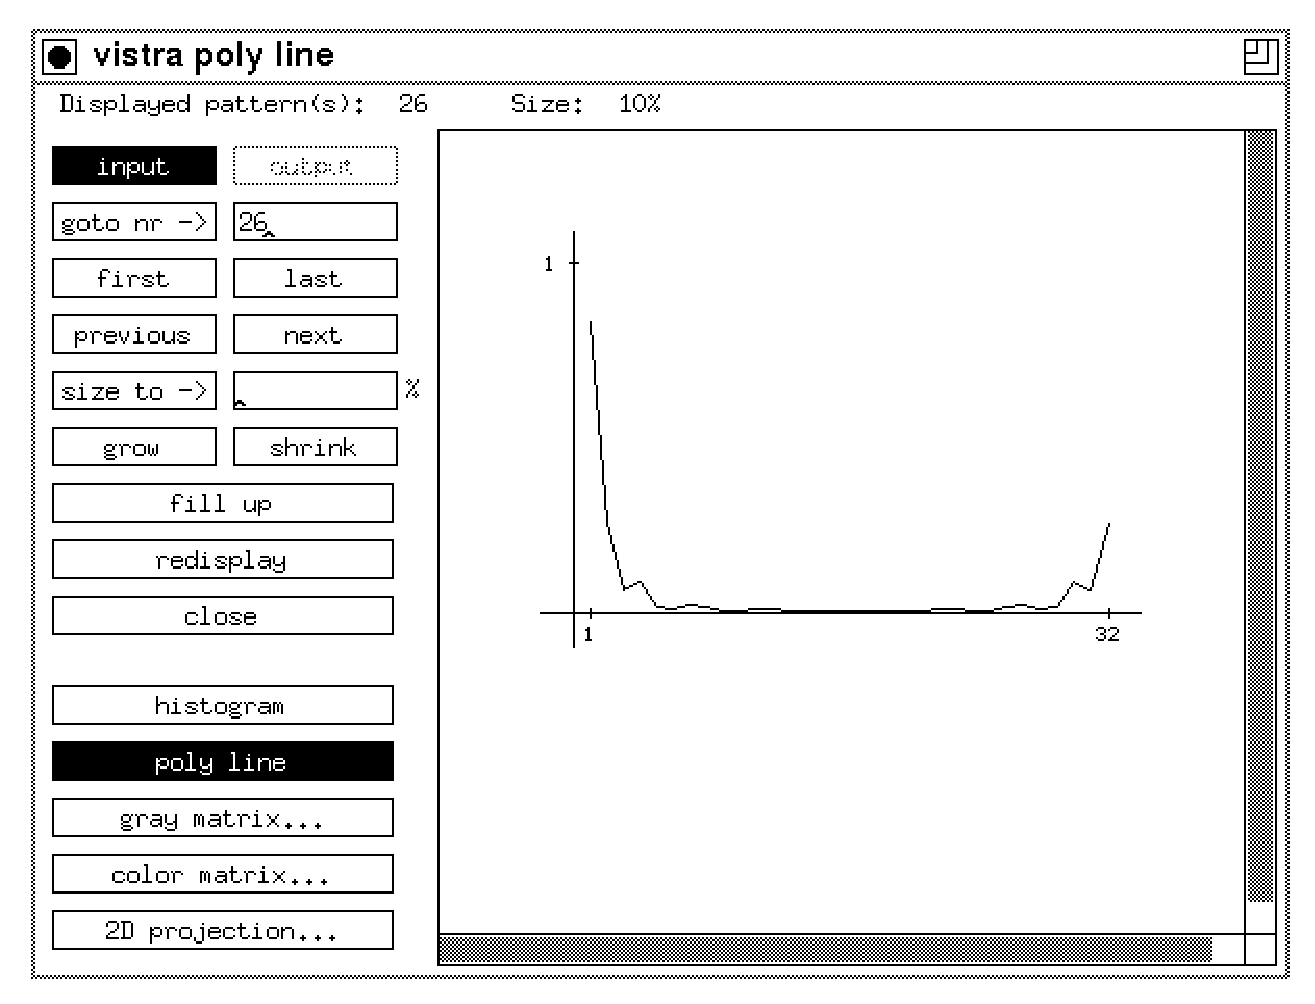
\psfig{file=poly.ps,width=\textwidth,height=10cm}}
\caption{\label{poly} Linienzug-Darstellung eines Vektors}
\end{figure} 

Die x-Achse kann "uber die entsprechenden Buttons des Graphik-Fensters
gedehnt oder geschrumpft werden.
Eine L"angeneinheit der x-Achse ist im Minimalfall genau ein Pixel breit. 

\subsubsection*{Grauwertbild}

Abbildung~\ref{grayMat} zeigte bereits ein Grauwertbild eines Vektors.
Der dargestellte Vektor besitzt 256 Dimensionen, die in eine Matrix
mit 16~Zeilen und 16~Spalten eingeteilt wurden.
Jedes Vektorelement wird durch ein Quadrat repr"asentiert, das in einem
bestimmten Grauton gezeichnet ist.
Das kleinste Element aller Eingabevektoren (bzw.~Ausgabevektoren)
erh"alt dabei die geringste Intensit"at und wird daher schwarz dargestellt.
Das gr"o"ste Element erh"alt die h"ochste Intensit"at und erscheint wei"s.
Werte dazwischen werden je nach Gr"o"se in einem Grauton dargestellt. 

Die Anzahl der Zeilen~bzw.~Spalten der Matrix wird vom Benutzer festgelegt. 
Die Anzahl der Zellen mu"s jedoch mindestens so gro"s wie die Dimensionalit"at
des abzubildenden Vektors sein.
Die ersten Elemente des Vektors werden durch die erste Zeile der Matrix
repr"asentiert, die n"achsten durch die zweite Zeile etc.
"`"Ubersch"ussige"' Zellen werden wei"s dargestellt. 

Die Elemente $v_{1}, \ldots, v_{7}$ eines 7-dimensionalen Vektors w"urden
wie folgt auf eine 3x3-Matrix verteilt werden:

\hspace*{2cm}
\begin{tabular}{|c|c|c|}
\hline $v_{1}$ & $v_{2}$ & $v_{3}$ \\
\hline $v_{4}$ & $v_{5}$ & $v_{6}$ \\
\hline $v_{7}$ & & \\ \hline
\end{tabular}    
 
Die Gr"o"se der quadratischen Zellen kann "uber die entsprechenden Buttons
des Graphik-Fensters ver"andert werden.
Die Minimalgr"o"se betr"agt ein Pixel. 

\subsubsection*{Farbbild}

Die Darstellung eines Vektors als Farbbild erfolgt analog der
Grauwert-Darstellung.
Einziger Unterschied ist die Verwendung des gesamten Farbspektrums
anstelle von Graut"onen.

\subsubsection*{2D-Projektion}

Die 2D-Projektion ist die einzige Darstellungsart, in der
{\it alle} Vektoren in einer einzigen Graphik wiedergegeben sind.
Jeder Vektor wird als ein Punkt in ein zweidimensionales Koordinatensystem
eingetragen.
Der Benutzer legt fest, welche Dimension der Vektoren die x-Werte und
welche die y-Werte liefert.

Abbildung~\ref{proj2D} zeigt ein Beispiel, in dem die Dimensionen~2 und 1
von insgesamt 10~000 Vektoren abgebildet sind.
Die Gr"o"se des Schaubilds kann "uber die entsprechenden Buttons des 
Graphik-Fensters variiert werden.

\begin{figure}[ht]
\centerline{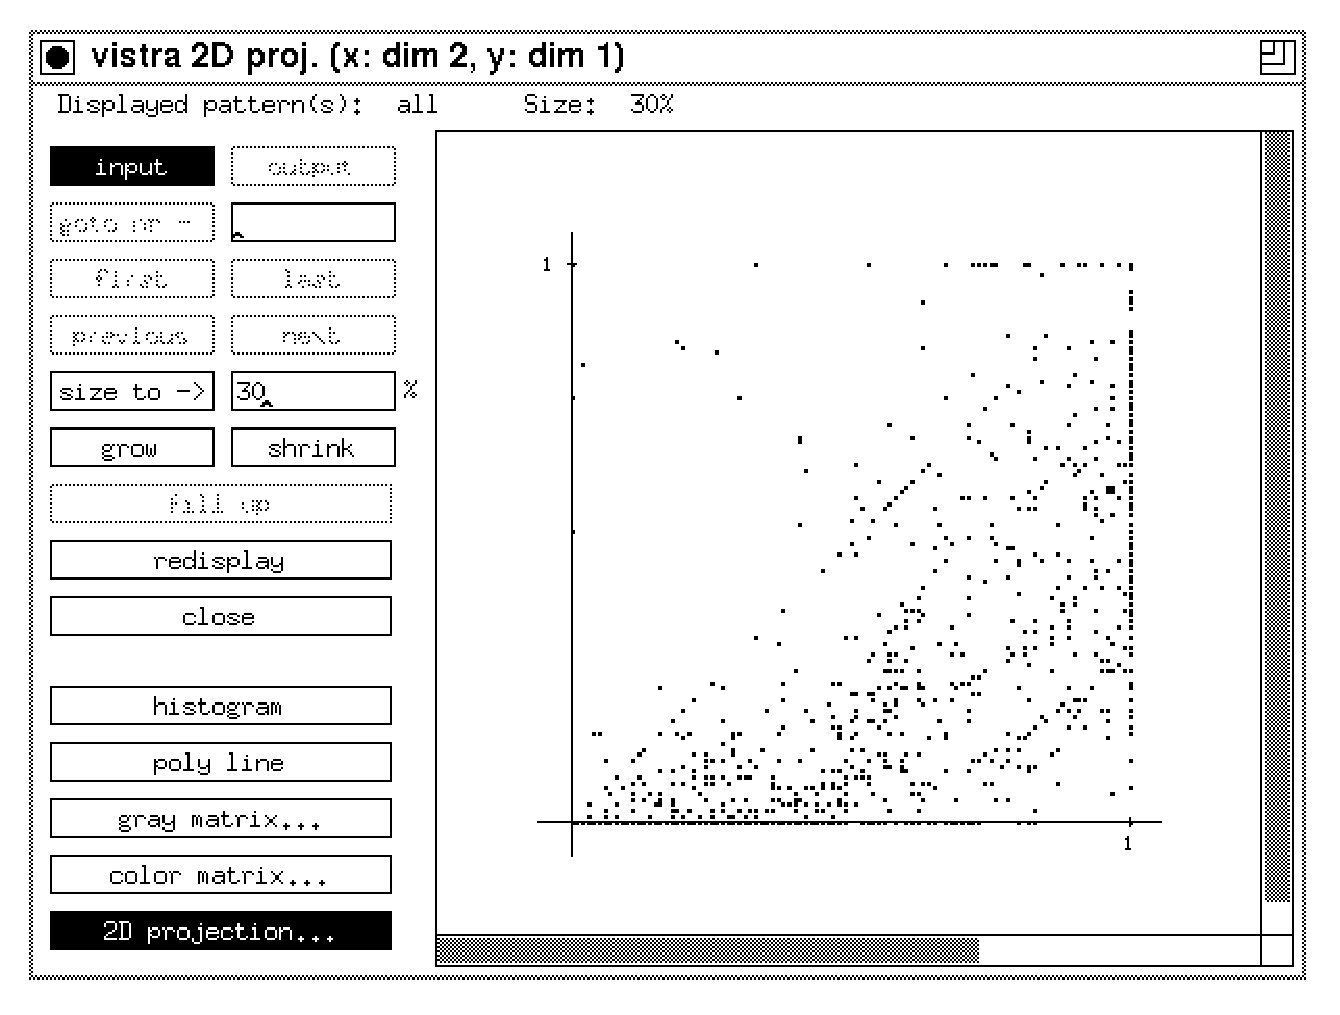
\psfig{file=proj2D.ps,width=\textwidth,height=10cm}}
\caption{\label{proj2D} Projektion zweier Dimensionen}
\end{figure}
 
\subsection{Das Statistik-Fenster}

Das Statistik-Fenster liefert allgemeine und statistische Informationen
"uber die geladenen Trainingsvektoren.
Abbildung~\ref{statistics} zeigt ein Beispiel.

\begin{figure}[ht]
\centerline{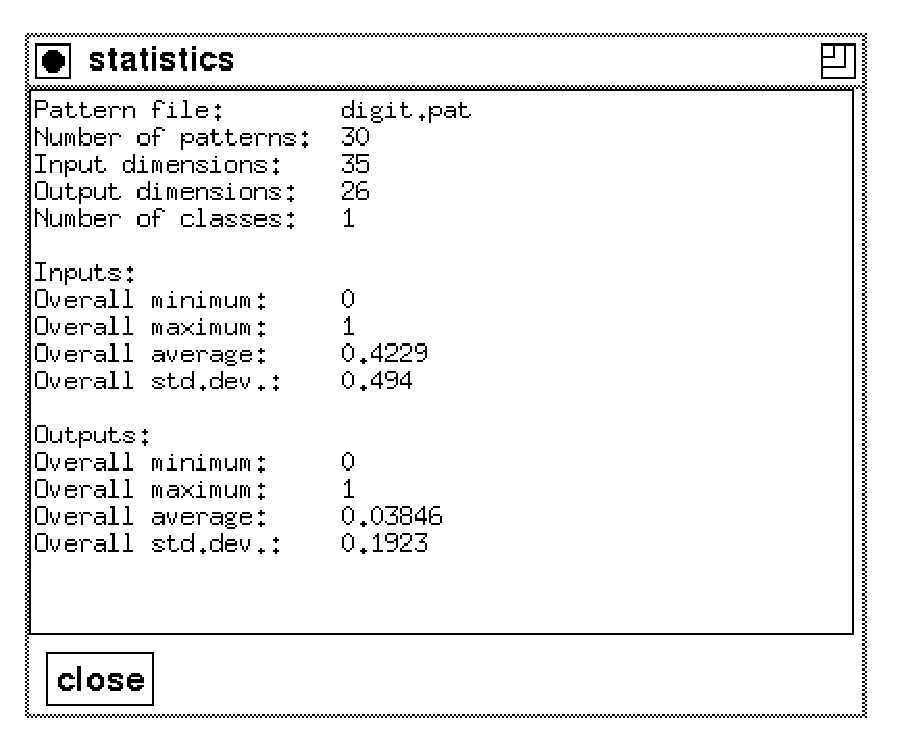
\psfig{file=stat.ps,width=10cm,height=8cm}}
\caption{\label{statistics} Das Statistik-Fenster}
\end{figure}

Der erste Teil zeigt allgemeine Informationen zu die Trainingsvektoren.
Die weiteren Abschnitte enthalten statistische Daten "uber 
die Eingabe- und Ausgabevektoren, wie sie auch "uber die "`Load"'-Men"us
des Hauptfensters berechnet werden k"onnen.  

Das Statistik-Fenster mu"s "uber "`close"' geschlossen werden, bevor
im Hauptfenster weitergearbeitet werden kann.

\subsection{Das Kovarianzmatrix-Fenster}

Das Kovarianzmatrix-Fenster zeigt eine Matrix, die alle Kovarianzen
zwischen je zwei Dimensionen der im Hauptfenster befindlichen Vektoren
enth"alt.
Stellt $nvecs$ die Anzahl der Vektoren und $ndims$ die Anzahl der
Dimensionen dar, so wird eine 
$ndims\times\/ndims$-Matrix $cov$ berechnet, in der das
Element $cov_{ij}$ die Kovarianz der Dimensionen $i$ und $j$ enth"alt. \\
Sei $avg_{i}$ der Mittelwert der Dimension $i$
($avg_{i} = \frac{1}{nvecs} \sum_{k=1}^{nvecs} v_{ki}$,  
$v_{k}$: $k$-ter Vektor), so berechnet sich $cov_{ij}$ wie folgt:

\[ cov_{ij} = \frac{1}{nvecs} \sum_{k=1}^{nvecs} 
(v_{ki} - avg_i)(v_{kj} - avg_j) 
\]    

F"ur $i=j$ erh"alt man aus obiger Formel:
\begin{displaymath}
cov_{ii} = \frac{1}{nvecs} \sum_{k=1}^{nvecs} 
(v_{ki} - avg_i)^{2}
\end{displaymath}
$cov_{ii}$ stellt also gerade die Varianz $\sigma^{2}_{i}$
der Dimension $i$ dar.
Die Matrix $cov$ ist au"serdem spiegelsymmetrisch, da f"ur alle $i,j$
gilt: $cov_{ij} = cov_{ji}$.

Abbildung~\ref{covariances} zeigt das Kovarianzmatrix-Fenster, das
die Kovarianzen f"ur folgende Vektoren enth"alt:

\nopagebreak
\begin{tabular}{l@{\hspace{1cm}}l}
{\sl Vektor~1:} & {\tt 0 2 1} \\
{\sl Vektor~2:} & {\tt 3 2 2} \\
{\sl Vektor~3:} & {\tt 1 2 3} \\
{\sl Vektor~4:} & {\tt 0 2 2} \\
\end{tabular}

\begin{figure}[ht]
\centerline{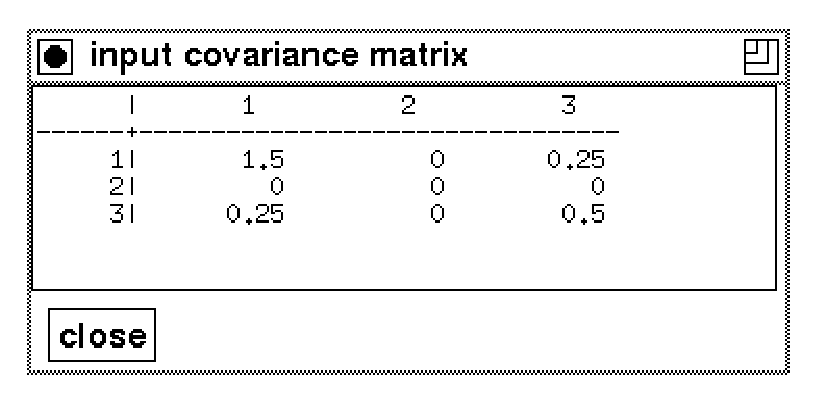
\psfig{file=cov.ps,width=8cm,height=4cm}}
\caption{\label{covariances} Das Kovarianzmatrix-Fenster}
\end{figure}

\subsection{Das Vektoren-Fenster}
\label{ssw}

Das Vektoren-Fenster kann nur ge"offnet werden, wenn Eingabe- und 
Ausgabevektoren vorhanden sind. 
Werden im Hauptfenster die Eingabevektoren (Ausgabevektoren) bearbeitet, 
so enth"alt das Vektoren-Fenster die Ausgabevektoren (Eingabevektoren).
Die Vektoren k"onnen im Vektoren-Fenster nur gelesen werden, 
Transformationen sind nur im Hauptfenster m"oglich.
Abbildung~\ref{vektorfenster} zeigt ein Vektoren-Fenster, in dem
momentan die Dimensionen 17 bis 22 der Vektoren 1 bis 22 angezeigt werden.
Der Titel des Fensters besagt, da"s es sich hierbei um die
Eingabevektoren handelt. 
"Uber den "`close"'-Button wird das Fenster wieder geschlossen. 

\begin{figure}[ht]
\centerline{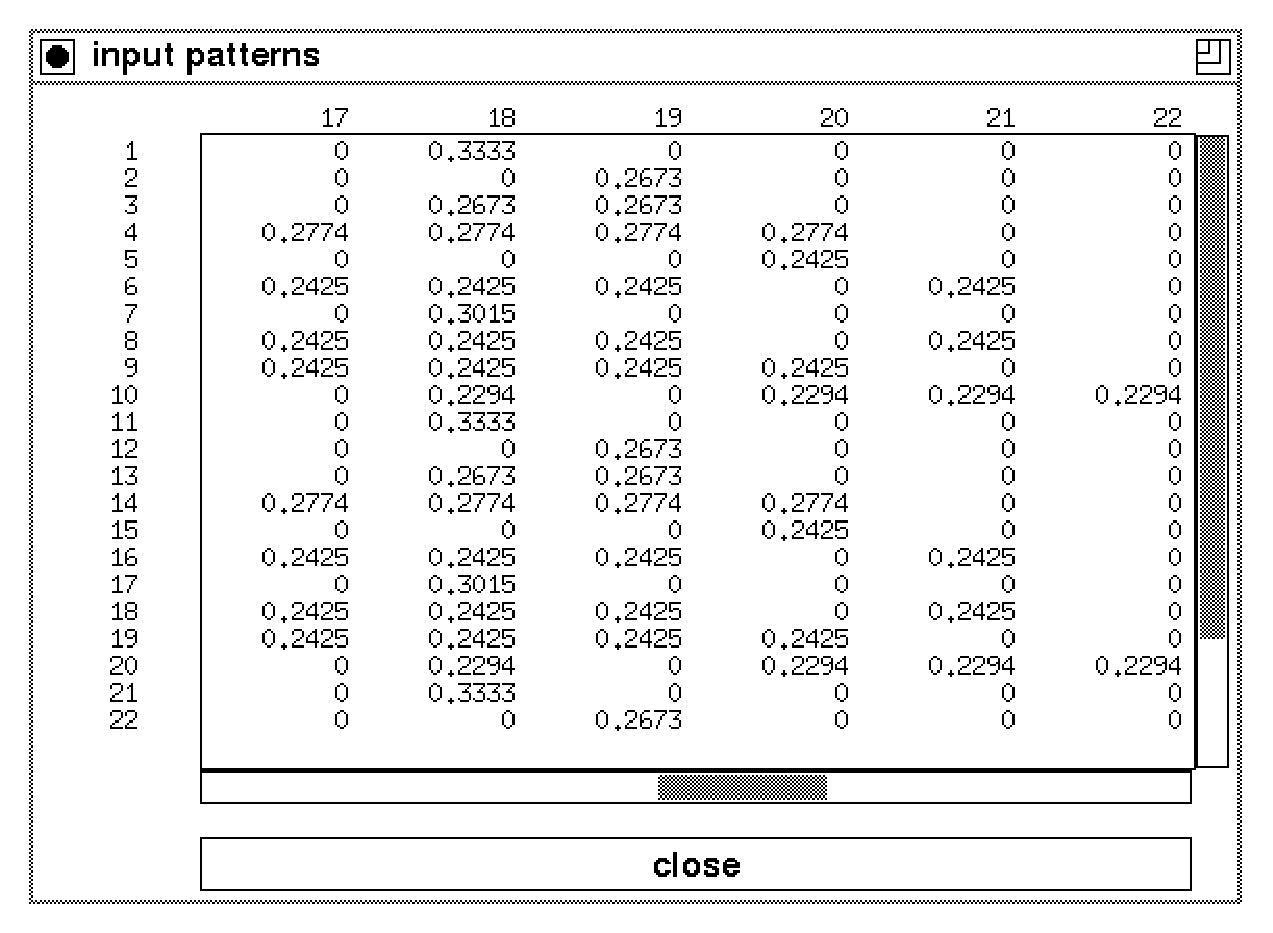
\psfig{file=readsh.ps,width=\textwidth,height=8cm}}
\caption{\label{vektorfenster} Das Vektoren-Fenster}
\end{figure}




